
\documentclass{unswmaths}
\usepackage{mathtools}
\usepackage{unswshortcuts}
\usepackage{fullpage}
\usepackage{float}
\usepackage{pgfplots}
\newcommand{\N}{\frac{\alpha(\alpha + b + \nu)}{\beta \left(\alpha - r\left[ 1 + \frac{\nu}{b + \gamma}\right] \right)}}
\newcommand{\X}{\frac{\alpha + b + \nu}{\beta}}
\newcommand{\Y}{\frac{r}{\alpha}\N}
\newcommand{\Z}{\frac{r}{\alpha}\left( \frac{\nu}{b + \gamma} \right)\N}
\author{Adam J. Gray}
\studentno{3329798}
\subject{Biomathematics}
\title{Assignment 1}


\begin{document}

\unswtitle

\section*{Question 1}
\subsection*{a}
	$ F $ is a linear combination of $ N $ and $ \frac{dN}{dt} $. This means that the larger the population is the more demand for the food there is. It also means that the faster the populations is growing, the more demand for food there is which would make sense because cell division could require \emph{more resources}.
\subsection*{b}
	\begin{align*}
		\frac{dN}{dt} &= rN \frac{T - \left(c_1N + c_2\frac{dN}{dt}\right)}{T} \\
		\frac{dN}{dt} \left( 1 + \frac{rc_2N}{T}\right) &= rN\left(1 - \frac{c_1N}{T} \right) \\
		\frac{dN}{dt} &= rN \left( \frac{\frac{T}{c_1} - N}{\frac{T}{c_1} + \frac{rc_2N}{c_1}} \right) \\
			&= rN \left( \frac{K - N}{K + aN}\right)
	\end{align*}
	where $ K = \frac{T}{c_1} $ and $ a = \frac{rc_2}{c_1} $.
\subsection*{c}
	Let $ f(N) = rN\left( \frac{K-N}{K+aN} \right) $ thus $ f(N) = 0 \Longrightarrow N^* = 0, N^* = K $.
	\begin{align*}
		f'(N) = r \left( \frac{K-N}{K+aN} \right) + rN \left( \frac{-(K+aN) - (K-N)a}{(K+aN)^2}\right)
	\end{align*}
	and
	\begin{align*}
		f'(0) &= r > 0 \\
		f'(K) &= \frac{-r}{a+1} < 0
	\end{align*}
	thus the steady states are $ N = 0 $ and $ N = k $ and they are unstable and stable respectively.
\section*{Question 2}
\subsection*{a}
	\begin{align*}
		\frac{dx}{dt} = 0 &\Longrightarrow 0.2x\left( 1 - \frac{x}{3} \right) = 0 \\
			& \Longrightarrow x^* = 0, 3
	\end{align*}
	So the steady states of the system are $ x^* = 0 $ and $ x^* = 3 $.
\subsection*{b}
	\begin{align*}
		\frac{dx}{dt} &= 0.2x\left( 1 - \frac{x}{3} \right) \\
		\int \frac{dx}{x(3-x)} &= \frac{1}{15} \int dt \\
		\int \frac{dx}{3x} + \int \frac{dx}{3(3-x)} &= \frac{1}{15} \int dt \\
		\frac{1}{3} \ln(x) - \frac{1}{3} \ln(3-x) &= \frac{t}{15} + C \\
		\ln \left( \frac{x}{3-x} \right) &= \frac{t}{5} + B \\
		\frac{x}{3-x} &= \exp(\frac{t}{5} + B) \\
		x &= \frac{3\exp(\frac{t}{5} + B)}{1 + \exp(\frac{t}{5} + B)}
	\end{align*}
	As $ x(0) = x_0 $
	\begin{align*}
		B &= \ln \left( \frac{x_0}{3-x_0} \right)
	\end{align*}
	and so
	\begin{align*}
		x = \frac{3 x_0 \exp(\frac{t}{5})}{3 + x_0 (\exp(\frac{t}{5}) - 1)}.
	\end{align*}
\subsection*{c}
	The steady states of the population are
	$ x^* = 0 $ and $ x^* = 3 - 15E $. Note that the second steady state is a function of $ E $ and for a sustainable yield we would require $ E < \frac{1}{5} $ so that the steady state is positive.
	
\subsection*{d}
	As per the last section the maximum sustainable yield is $ E = \frac{1}{5} $.
    We can also justify this by finding the largest $ E $ for which $ 0.2(1- x / 3) = E $ has a solution. 
\section*{Question 3}
\subsection*{a}
Let $ H : [0, \infty) \lra \mathbb{R} $ be defined as
\begin{align*}
    H(t) = 
    \begin{cases}
        h & t \mod 12 \leq T \\
        0 & \text{ otherwise }
    \end{cases}
\end{align*}
where $ h $ is the harvesting quantity. 
Then the governing equation would be
\begin{align*}
    \frac{dF}{dt} = aF(t) - cF^2(t) - H(t)
\end{align*}
where $ F(t) $ is the population of fish at time $ t $ (months) and $ r $ is the population growth rate in fish per month.
\subsection*{b}
\begin{figure}[H]
    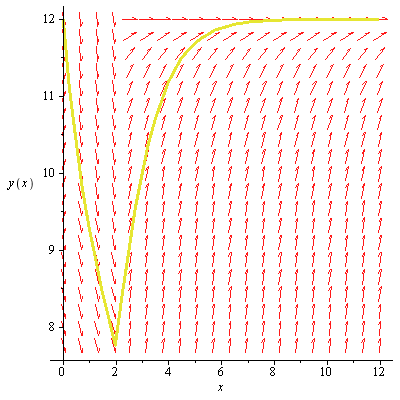
\includegraphics[scale=0.3]{population_2}
    \caption{$T=2$}
\end{figure}

\begin{figure}[H]
    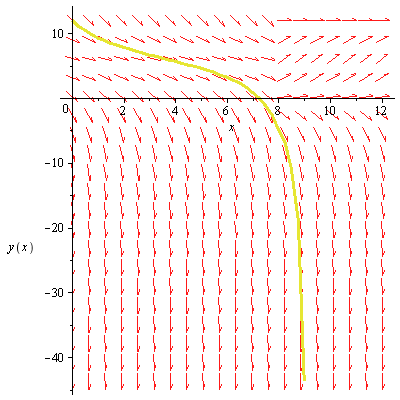
\includegraphics[scale=0.3]{population_8}
    \caption{$T=8$}
\end{figure}
Clearly when $ T = 8 $ the population collapses, whereas this is not the case with $ T = 2 $. 
\section*{Question 4}
\subsection*{a}
The coefficient $ 2a $ steers the system in the sense that for $ a = 0 $ the system models a commensalistic symbiotic relationship. That is one party, $ x $, benefits without harm to the other party, $ y $. 
As $ a $ increases this scales into a mutualistic relationship where both parties benefit. For values of $ a > 1 $ we would actually have $ y $ benefiting \emph{more} from the relationship, than $ y $ does. 
\subsection*{b}
The nontrivial steady state is at $ x = 6 / (1 - 4a) $, $ y = -1 - 3 / (4a - 1) $. Now if we want the non-trivial steady state to be in the population quadrant we need $ x > 0 $ and $ y > 0 $.
    For $ x > 0 $ we need $ a < 1 / 4 $. For $ y > 0 $ we need  $ a > -1/2 $.  To prevent explosive growth we would need $ a < 1/4 $.
\begin{figure}[H]
    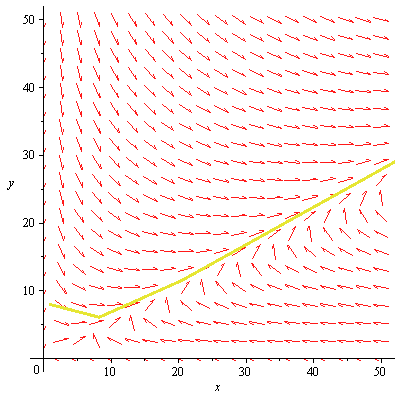
\includegraphics[scale=0.3]{dir_field_1_3}
    \caption{$ a= 1 / 3 $}
\end{figure}

\begin{figure}[H]
    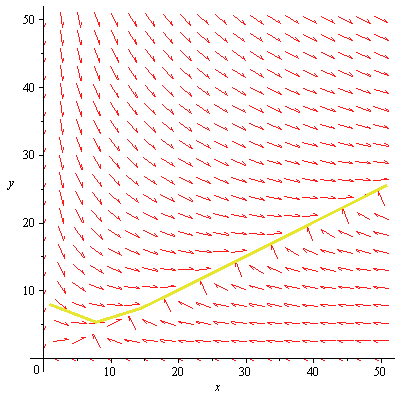
\includegraphics[scale=0.3]{dir_field_1_4}
    \caption{$ a= 1 / 4 $}
\end{figure}

\begin{figure}[H]
    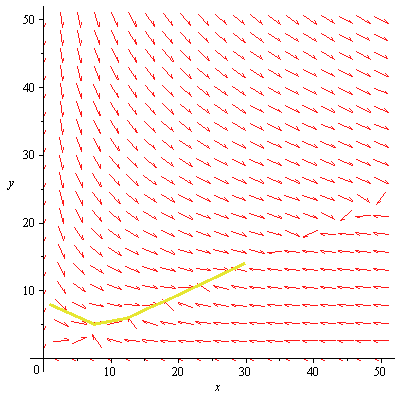
\includegraphics[scale=0.3]{dir_field_1_5}
    \caption{$ a= 1 / 5 $}
\end{figure}
\section*{Question 5}
\subsection*{a}
Clearly there is a steady state at $ x=0=y $.  Also there is a steady state at $ y = 0, x = K $. 

There is also a steady state at $ x = c / d $ and $ y = a / b - ac / bdK $. 
This is the non-trivial steady state.
Note that
\begin{align*}
    J &= \left[ \begin{array}{cc} a - 2a x / K - by & -bx \\ dy & -c + dx \end{array}\right] \\
    J \big|_{x = c/d, y = a(1/b - c/bdK} &= \left[ \begin{array}{cc} -ac / dK & -bc / d \\ ad / b - ac /bK & 0 \end{array} \right].
\end{align*}
Now 
\begin{align*}
    \operatorname{Tr}\left( J \big|_{x = c/d, y = a(1/b - c/bdK} \right) &= \frac{-ac}{dK}  \\
    \operatorname{det}\left(  J \big|_{x = c/d, y = a(1/b - c/bdK} \right) &= ac\left( 1 - c / dK \right).
\end{align*}
Assuming that all constants are positive this means that the non-trivial steady state is stable if $ c/dK < 1 $. 
\section*{b}
In the following plots $ x - $ purple $ y- $ blue.
\begin{figure}[H]
    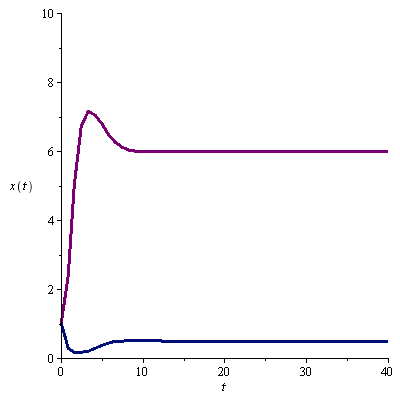
\includegraphics[scale=0.5]{pp_1_1}
    \caption{$x(0)=1,y(0)=1$}
\end{figure}
\begin{figure}[H]
    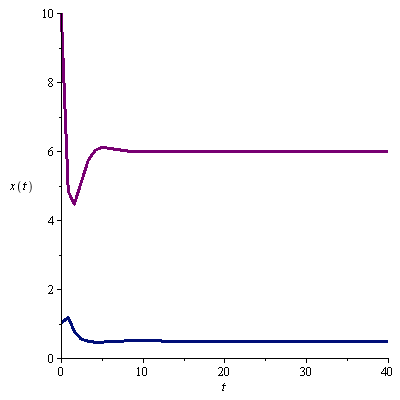
\includegraphics[scale=0.5]{pp_10_1}
    \caption{$x(0)=10,y(0)=1$}
\end{figure}
\begin{figure}[H]
    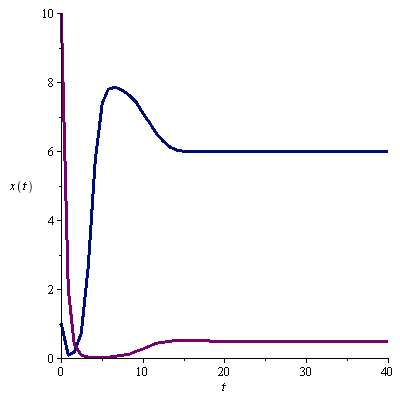
\includegraphics[scale=0.5]{pp_1_10}
    \caption{$x(0)=1,y(0)=10$}
\end{figure}
\section*{Question 6}
\subsection*{a}
$ r_MS_MI_F $ is the term which describes the rate at which males leave the susceptible state because they have become infected due to a male - female interaction.

$ a_MI_M $ is the tern which describes how quickly males recover from the infected state and become susceptible again. Note that in this model there is no period of conferred immunity and infected individuals simply become susceptible again.

\subsection*{b}
Clearly adding equations 1 and 3 and 2 and 4 yields 0 in each case. 

As we can write $ S_F = N_F - I_F $ and $ S_M = N_M - I_M $ we can substitute these into equations 3 and 4 to get
\begin{align*}
    \frac{dI_M}{dt} &= r_MI_F(N_M-I_M)-a_MI_M \\
    \frac{dI_F}{dt} &= r_FI_M(N_F - I_F) - a_FI_F.
\end{align*}
Note that this completely determines the system because $ \frac{dS_M}{dt} = -\frac{dI_M}{dt} $ and  $ \frac{dS_F}{dt} = -\frac{dI_F}{dt} $.
\subsection*{c}
The threshold population must exist at an equilibrium. Solving for the equilibriums we get that
\begin{align*}
    N_F &= I_F - \frac{a_FI_F}{r_FI_M} \\
    N_M &= I_M - \frac{a_MI_M}{r_MI_F}
\end{align*}
and taking the product of these we get that
\begin{align*}
    N_MN_F &= \left( \frac{I_F + a_FI_F}{r_FI_M} \right) \left( I_M + \frac{a_MI_M}{r_MI_F} \right) \\
        &= I_FI_M + \frac{a_Ma_F}{r_Mr_F} + \frac{a_MI_M}{r_M} + \frac{a_fI_F}{r_F} \\
        &\geq  \frac{a_Ma_F}{r_Mr_F} 
\end{align*}
because all the other terms must be positive if we are at (or above) the threshold population.
\section*{Question 7}
\subsection*{a}
\begin{align*}
    \frac{dX}{dt} &= \underbrace{a(X+Y+Z)}_{\text{natural birth rate}} + \underbrace{\gamma Z}_{\text{re-susceptible rate}} - \underbrace{\beta XY}_{\text{infection rate}} - \underbrace{bX}_{\text{natural death rate}} \\
    \frac{dY}{dt} &= \underbrace{\beta XY}_{\text{infection rate}} - \underbrace{(\alpha + b)Y}_{\text{death rate}} - \underbrace{\nu Y}_{\text{recovery rate}} \\
    \frac{dZ}{dt} &= \underbrace{\nu Y}_{\text{recovery rate}} - \underbrace{bZ}_{\text{natural death rate}} - \underbrace{\gamma Z}_{\text{re-susceptible rate}}
\end{align*}
\subsection*{b}
    Subbing the equations in the question we get that
    \begin{align*}
        & X(a-b) + Z(\gamma + a) + aY - \beta XY\\ 
&= \X(a+b) + \Z(\gamma + a) + a\Y \\
& \ \ \ - \beta\X\Y \\
&= r\X + \frac{r\nu(\alpha + b + \nu)}{(b+\gamma)\beta\alpha - \beta r(b +\gamma + \nu)} +
\frac{ar(\alpha + b + \nu)(b + \gamma)}{\beta\alpha (b + \gamma) - \beta r ( b + \gamma) + \beta r \nu} \\
& \ \ \ - \frac{(\alpha + b + \nu)^2(b+\gamma)}{\beta\alpha(b + \gamma) + \beta r(b + \gamma) + \beta r \nu} \\
&= \frac{r}{\beta}\left[(\alpha + b + \nu)- (\alpha + b + \nu)\right] \\
&= 0
\end{align*}
\begin{align*}
    &\beta X Y - (\alpha + b) Y - \nu Y \\
    &= \beta \X\Y - (\alpha + b)\Y - \nu \Y \\
    &= \frac{r(\alpha + b + \nu)^2(b + \gamma)}{\alpha\beta(b + \gamma) - \beta r (b + \gamma) - \beta r \nu} 
- \frac{r(\alpha + b)(\alpha + b + \nu)(b + \gamma)}{\beta \alpha(b + \gamma)- \beta r (b + \gamma) - \beta r \nu } 
- \frac{\nu(b + \gamma) r(\alpha + b + \nu)}{\beta \alpha(b + \gamma) -  \beta r (b + \gamma) - \beta r \nu } \\
    &= \frac{r(\alpha+b + \nu)}{\alpha \beta - \beta r (b + \gamma) - \beta r \nu} \left[ (\alpha + b + \nu)(b + \gamma) - (\alpha + b)(b+\gamma) - \nu(b + \gamma)\right] \\
    &= 0
\end{align*}
\begin{align*}
    & \nu Y - b Z - \gamma Z \\
    &= \nu \Y - b \Z - \gamma \Z \\
    &= \frac{r\nu(\alpha + b + \nu)}{\beta\left(\alpha - r\left[ 1 + \frac{\nu}{b + \gamma} \right] \right)} \left( 1 - \frac{b + \gamma}{b + \gamma}\right) \\
    &= 0
\end{align*}
Do the values given in the question are in fact a steady state for the system.
\subsection*{c}
Note that $ N_2 = X_2 + Y_2 + Z_2 $ and so we can view $ N_2 $ as the equilibrium population. Therefor if
\begin{align*}
    \alpha < r\left( 1 + \frac{\nu}{b + \gamma}\right)
\end{align*}
then this population is negative which does not make sense. If equality hold then the population is infinite, which is more like saying there is no equilibrium population.

In that context Anderson and May's remarks make sense in that the disease can regulate the population size. I think that this is a really interesting result because it means that a population's size can be \emph{capped} without appealing to logistic growth arguments, but rather just to the existence of a pathogen with a sufficiently high death rate.
\section*{Question 8}
\subsection*{a}
    \begin{align*}
        \underbrace{\frac{dx}{dt}}_{animals\cdot km^{-2} \cdot day^{-1}} = \underbrace{a}_{day^{-1}}\underbrace{x}_{animals \cdot km^{-2}} - \underbrace{b}_{animals^{-1} \cdot km^{2} \cdot day^{-1}}\underbrace{xy}_{animals^{2} \cdot km^{-4}} \\
        \underbrace{\frac{dy}{dt}}_{animals\cdot km^{-2} \cdot day^{-1}} = -\underbrace{c}_{day^{-1}}\underbrace{y}_{animals \cdot km^{-2}} + \underbrace{d}_{animals^{-1} \cdot km^{2} \cdot day^{-1}}\underbrace{xy}_{animals^{2} \cdot km^{-4}} \\
    \end{align*}
\subsection*{b}
     \begin{align*}
        \frac{dx(t)}{c} &\sim \frac{animals^{-1} \cdot km^2 \cdot days^{-1} animals \cdot km^{-2}}{days^{-1}} &\sim unitless \\
        \frac{by(t)}{a} &\sim \frac{animals^{-1} \cdot km^2 \cdot days^{-1} animals \cdot km^{-2}}{days^{-1}} &\sim unitless \\
        at &\sim days^{-1} \cdot days &\sim unitless \\
        \frac{c}{a} &\sim \frac{days^{-1}}{days^{-1}} &\sim unitless
     \end{align*}
\subsection*{c}
    Chain rule:
    \begin{align*}
        \frac{du}{d\tau} = \frac{du}{dt} \frac{dt}{d\tau} = \frac{d}{ca}\frac{dx}{dt} \\
        \frac{dv}{d\tau} = \frac{dv}{dt} \frac{dt}{d\tau} = \frac{b}{a^2} \frac{dy}{dt} \\
    \end{align*}
    Subbing in:
    \begin{align*}
        \frac{du}{d\tau} &= \frac{d}{ca} \left( ax + bxy \right) \\
            &= \frac{d}{ca} \left( \frac{ac}{d} u + \frac{bca}{db} v\right)u \\
            &= u(1-v) \\
        \frac{dv}{d\tau} &= \frac{d}{a^2} \left( -cy + dxy \right) \\
            &= \frac{d}{a^2} \left( \frac{-ca}{b} v + d\frac{bca}{db} vu\right) \\
            &= \frac{c}{a} v\left(u - 1\right) \\
            &= \alpha v(u - 1)
    \end{align*}
    Equilibrium points:
    \begin{align*}
        \frac{du}{d\tau} = u(1-v) = 0 \Longrightarrow  u = 0 \text{ or } v = 0 \\
        \frac{dv}{d\tau} \alpha v(u-1) = 0 \Longrightarrow v = 0 \text{ or } u = 1 \\
    \end{align*}
    For equilibriums $ u = 0 \Longrightarrow v = 0 $ and $ v = 1 \Longrightarrow u = 0 $.
    Thus equilibriums are at $ (0,0) $ and $ (1,1) $.
\subsection*{d}
    \begin{align*}
        \frac{dv}{du} &= \frac{dv}{dt} \frac{dt}{du} \\
            &= \frac{\alpha v(u-1)}{u(1-v)}
    \end{align*}
    Integrating:
    \begin{align*}
        \int \frac{(1-v)}{v}dv &= \alpha \int \frac{(1-u)}{u} du \\
        \ln(v) - v &= \alpha \ln(u) - \alpha u + C \\
        \ln(v) - v &= -\ln(u^\alpha) + \alpha u  + C \\
        \ln(u^\alpha v) - v -\alpha u &= C
    \end{align*}
    Equivalently
    \begin{align*}
        \ln(u^\alpha v) - v -\alpha u &= C
    \end{align*}
\subsection*{e}
\begin{figure}[H]
    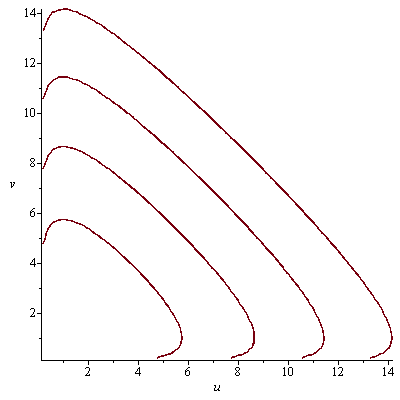
\includegraphics[scale=0.5]{orbits_1}
    \caption{$\alpha = 1$}
\end{figure}
\begin{figure}[H]
    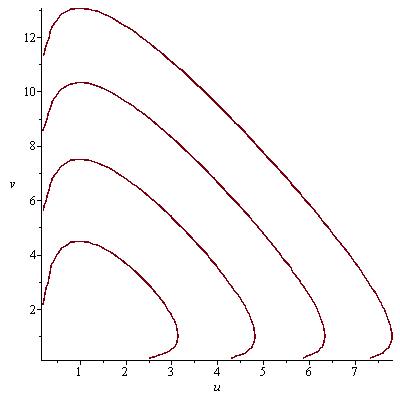
\includegraphics[scale=0.5]{orbits_2}
    \caption{$\alpha = 2$}
\end{figure}
\begin{figure}[H]
    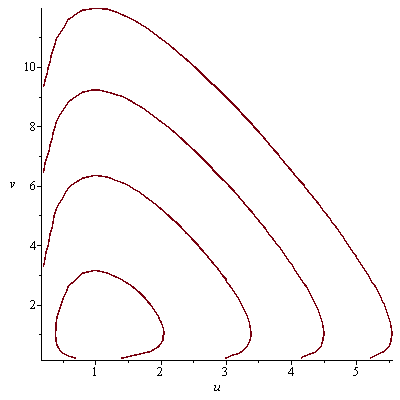
\includegraphics[scale=0.5]{orbits_3}
    \caption{$\alpha = 3$}
\end{figure}
\subsection*{f}
    Differentiating:
    \begin{align*}
        \frac{dC}{du} &= -\frac{1}{u^\alpha v} ( \alpha u^{\alpha-1} v ) + \alpha \\
        \frac{dC}{dv} &= -\frac{1}{u^\alpha v} + 1
    \end{align*}
    Stationary points:
    \begin{align*}
        -\frac{1}{u^\alpha v} ( \alpha u^{\alpha-1} v ) + \alpha = 0 \Longrightarrow u = 1 \\
        -\frac{1}{u^\alpha v} + 1 = 0 \Longrightarrow u^\alpha v = 1 \Longrightarrow v = 1
    \end{align*}
    Only one stationary point so this \emph{must} be the minimum. 
    
    Minimum at $ (1,1) $ with value $ 1 + \alpha $ (by simple substitution).
\section*{Question 9}
\subsection*{a}
\begin{figure}[H]
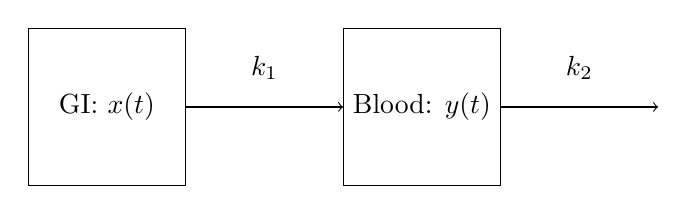
\begin{tikzpicture}
    \draw (0,0) -- (0,2) -- (2,2)  -- (2,0) -- (0,0);
    \draw[->] (2,1) -- (4,1);
    \draw (4,0) -- (4,2) -- (6,2) -- (6,0) -- (4,0);
    \draw[->] (6,1) -- (8,1);
    \draw (1,1) node {GI: $ x(t) $};
    \draw (5,1) node {Blood: $ y(t) $};
    \draw (3,1.5) node {$k_1$};
    \draw (7,1.5) node {$k_2$};
\end{tikzpicture}
\end{figure}

The system of differential equations is given by
\begin{align*}
    \left( \begin{array}{c} \frac{dx}{dt} \\ \frac{dy}{dt} \end{array}\right) &= \left[ \begin{array}{cc} -k_1 & 0 \\ k_1 & -k_2 \end{array} \right] \left( \begin{array}{c} x(t) \\ y(t) \end{array}\right)
\end{align*}
along with the initial conditions
\begin{align*}
    x(0) &= A \\
    y(0) &= 0 
\end{align*}
\subsection*{b}
Let
\begin{align*}
   B := \left[
        \begin{array}{cc}
            -k_1 & 0 \\
            k_1 & - k_2
        \end{array}
        \right].
\end{align*}
It is clear to see that this has eigenvalues $ \lambda_1 = -k_1 $ and $ \lambda_2 = -k_2 $. Simple computations show that the corresponding eigenvectors are
\begin{align*}
    \mathbf{v}_1 &= \left( \begin{array}{c} 1/k_1 \\ 1/(k_2-k_1) \end{array}\right) \\
    \mathbf{v}_2 &= \left( \begin{array}{c} 0 \\ 1 \end{array}\right)  
\end{align*}
and so the general solution to the system of differential equations is
\begin{align*}
    \left( \begin{array}{c} x(t) \\ y(t) \end{array} \right) = \alpha \left( \begin{array}{c} 1/k_1 \\ 1/(k_2 - k_1) \end{array}\right) e^{-k_1 t} +  \beta \left( \begin{array}{c} 0 \\ 1 \end{array}\right) e^{-k_2 t}.
\end{align*}
By applying the initial conditions we get that system of equations
\begin{align}
    \alpha \left( \begin{array}{c} 1 / k_1 \\ 1 / (k_2 - k_1) \end{array} \right) + \beta \left( \begin{array}{c} 0 \\ 1 \end{array} \right) = \left( \begin{array}{c} A \\ 0 \end{array}\right)
\end{align}
which gives us that $ \alpha = k_1 A $ and $ \beta = -k_1 A / (k_2 - k_1 ) $.
So the solutions look like
\begin{figure}[H]
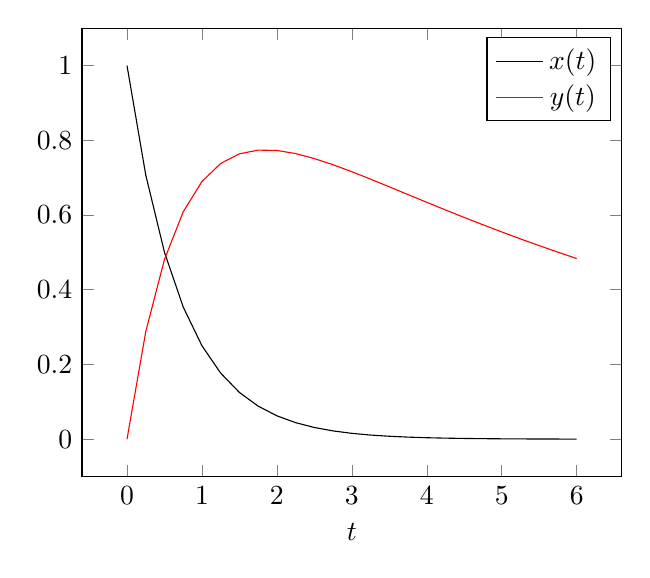
\begin{tikzpicture}
    \begin{axis}[
        xlabel = $t$
    ]
    \addplot[domain=0:6] {exp(-1.386*x};
    \addplot[domain=0:6,color=red] {-1.1111 * exp(-1.386 * x) + 1.1111 * exp(-0.1386 * x)};
    \addlegendentry{$x(t)$}
    \addlegendentry{$y(t)$}
    \end{axis}
\end{tikzpicture}

Decongestant levels quickly drop in the GI tract but they build up quickly in the blood and are slow to clear from the blood.
\end{figure}
\end{document}
